\slajdid{02-s034}
\begin{frame}[label=02-s034]
\gusttekst
\alert{Osnova minimizacije putem Karnoovih tabela i jesu specifično napravljene tabele u kojima je lako uočiti proizvode ili zbirove sa Hemingovim rastojanjem 1.}

\begin{columns}[c,onlytextwidth]
\begin{column}{.60\textwidth}
Tabela sa 1 promenljivom

% Oblici 2x1/1x2 nisu standardni šabloni paketa karnaugh-map.
% Indeksi vertikalnog primera namerno su 1,0 kao u originalu.
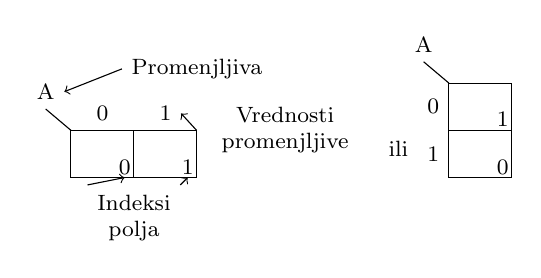
\begin{tikzpicture}[font=\fontsize{8}{9.5}\selectfont,x=8mm,y=6mm]
\draw (0,0) rectangle (2,1) (1,0)--(1,1);
\draw (0,1)--(-.4,1.45) node[above] (a) {A};
\node[above] at (.5,1) (v0) {0};\node[above] at (1.5,1) (v1) {1};
\node[anchor=south east,inner sep=1pt] at (1,0) (i0) {0};
\node[anchor=south east,inner sep=1pt] at (2,0) (i1) {1};
\node at (2.0,2.3) (prom) {Promenjljiva};
\draw[->] (prom.west)--(a.east);
\node[align=center,text width=20mm] at (3.4,1.0) (val) {Vrednosti\\promenjljive};
\draw[->] (val.west)--(v1.east);
\node[align=center] at (1,-.85) (ind) {Indeksi\\polja};
\draw[->] (ind.north west)--(i0.south);
\draw[->] (ind.north east)--(i1.south);
\node at (5.2,.6) {ili};
\draw (6,0) rectangle (7,2) (6,1)--(7,1);
\draw (6,2)--(5.6,2.45) node[above] {A};
\node[left] at (6,1.5) {0};\node[left] at (6,.5) {1};
\node[anchor=south east,inner sep=1pt] at (7,1) {1};
\node[anchor=south east,inner sep=1pt] at (7,0) {0};
\end{tikzpicture}


Tabela sa 2 promenljive

% Poređenje 2x2, 1x4 i 4x1; crvene ivice zadržavaju izvorno isticanje.
\begin{tikzpicture}[font=\fontsize{8}{9.5}\selectfont,x=6.5mm,y=5.5mm]
\draw (0,2) rectangle (2,4) (1,2)--(1,4) (0,3)--(2,3);
\draw (0,4)--(-.5,4.5) node[above right] {A} node[below left] {B};
\foreach \x/\lab in {.5/0,1.5/1}{\node[above] at (\x,4) {\lab};}
\foreach \y/\lab in {3.5/0,2.5/1}{\node[left] at (0,\y) {\lab};}
\foreach \x/\y/\lab in {1/3/0,2/3/1,1/2/2,2/2/3}{\node[anchor=south east,inner sep=1pt] at (\x,\y) {\lab};}
\node[below] at (1,1.65) {1};
\node at (2.85,3.2) {ili};
\draw (4,0) rectangle (5,4);
\foreach \y in {1,2,3}{\draw (4,\y)--(5,\y);}
\draw (4,4)--(3.5,4.5) node[above left] {BA};
\foreach \y/\lab in {3.5/00,2.5/01,1.5/11,.5/10}{\node[left] at (4,\y) {\lab};}
\foreach \y/\lab in {3/0,2/1,1/3,0/2}{\node[anchor=south east,inner sep=1pt] at (5,\y) {\lab};}
\draw[DEcrvena] (4,0)--(5,0) (4,4)--(5,4);
\node[below] at (4.5,-.2) {2};
\node at (6.05,3.2) {ili};
\draw (7,3) rectangle (11,4);
\foreach \x in {8,9,10}{\draw (\x,3)--(\x,4);}
\draw (7,4)--(6.5,4.5) node[above right] {BA};
\foreach \x/\lab in {7.5/00,8.5/01,9.5/11,10.5/10}{\node[above] at (\x,4) {\lab};}
\foreach \x/\lab in {8/0,9/1,10/3,11/2}{\node[anchor=south east,inner sep=1pt] at (\x,3) {\lab};}
\draw[DEcrvena] (7,3)--(7,4) (11,3)--(11,4);
\node[below] at (9,2.65) {3};
\end{tikzpicture}

\end{column}
\begin{column}{.38\textwidth}
Uočite da indeksi kao i ranije odgovaraju vrednosti binarnog broja kojeg čine stanja promenljivih. Razlog zbog kojeg su indeksi odnosno stanja promenljivih prikazani na ovaj način je taj što sada susedna polja po indeksu imaju Hemingovo rastojanje 1. \alert{\underline{Susedna} \underline{polja} \underline{su} \underline{ona} \underline{koja} \underline{imaju} \underline{najmanje} \underline{jednu} \underline{zajedničku} \underline{stranicu.}} (u 2D prostoru to je jedna, dok će u 3D i 4D prostoru biti više zajedničkih stranica) U 1. Primeru je to zadovoljeno bez razmeštaja stanja promenljivih, dok je u 2. i 3. praktično raspored promenljivih preuređen.
\end{column}
\end{columns}
\end{frame}
